\chapter{Background and Motivation}
\renewcommand{\baselinestretch}{\mystretch}
\label{chap:bg}
%\setlength{\parindent}{0pt}



\section{Applications of DNA Sequencing}
There are a large number of motivations for sequencing DNA. In the medical field, genomics has applications in both research and applied medicine. One example where DNA sequencing has been used productively in applied medicine is for screening for the BRCA mutations. Through testing the BRCA1 and BRCA2 genes for mutations, it is possible to accurately predict if a patient is likely to develop cancer later in life. The US Preventative Services Task Force currently recommends screenings for women who are known to have a family history of breast cancer, around 2\% of the population \cite{USPSTF}. This type of application relies on exome sequencing, where only a small subsection of DNA is sampled to identify a risk factor for a certain disease. 

The research applications of sequencing have been clear for some time with  the Human Genome Project launching in 1990 \cite{HGP}.  With it's primary goals accomplished in 2003, this project has opened numerous areas for research, showing possible applications such as understanding genotypes of viruses for targeted treatments and also the advancement of other less related areas such as forensics. The sequencing of a full human genome also has significant impact on the nature of DNA sequencing, as it allows a much wider area of mapping sequencing. Mapping sequencing uses the fact that the structure of a piece of DNA is known in order to simplify the sequencing process. Exome sampling mentioned earlier is an example of this. 

DNA sequencing also plays an important role in ecology research where bio-diversity and historical biological characteristics can both be indicated by DNA samples and used to further current research. This field is particularly cost sensitive due to the enormous variety of DNA sampling that needs to be carried out and also presents some of the most complex problems for DNA sampling \cite{genomelength}.An example of this is the Polychaos Dubium which has 670 Giga base pairs (Gbp), dwarfing the size of the human genome at 3Gbp \cite{HGP2}. Due to the complexity of the operations we will see in the DNA sequencing process this presents important problems in sequencing \cite{parfrey2008dynamic}. Often this area often requires de novo sequencing techniques, using no prior knowledge of the genome in contrast to human samples where the general structure of the genome is known and can be used to simplify sequencing.  These de novo techniques present a significantly different problem set to exome sequencing where comparison against existing data is impossible.


Ecology research has significant practical applications within agriculture, where studies such as the sequencing of the Oil Palm genome are currently being undertaken in order to identify important genetic traits such as drought resistance and yield. It is in areas like these where fast sequencing of particularly long genetic sequences have practical applications, which acts as a driving motivation for producing a scalable architecture for this problem. Genetically Modified Organisms (GMO) are currently a growing trend in agriculture, with some companies in this area yielding over \$2Billion operating income per year \cite{Monsanto}.

In order to satisfy the growing demand for both full de novo sequencing and exome sequencing, there has been a large amount of research in the area. The result of this research is a large array of techniques and technologies designed to lower the cost and raise the speed of sequencing. In the last decade this has produced a significant advance with a set of Next Generation Sequencing technologies.




\section{The DNA Sequencing Process}
\subsection{The Structure of DNA}
Deoxyribonucleic acid is a molecule formed of four nucleotides (guanine, adenine, thymine, and cytosine), the structure of the molecule is a double helix with bonds formed between complementary pairs of nucleotides (guanine bonding with cytosine, adenine bonding with thymine) \cite{mandelkern1981dimensions}. These bonds are referred to as base pairs (bps) and are commonly used to quantify the size of the molecule. For example, the human genome is 3 billion base pairs long. The structure of DNA tends to be extremely long sequences. This structure has important ramifications on the sequencing techniques as discussed below.
\begin{figure}[h]
  \centering
  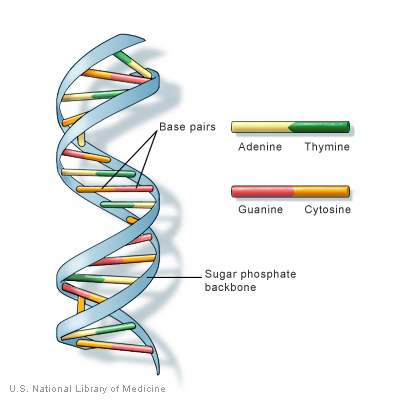
\includegraphics[width=0.45\textwidth]{./figs/dnastructure.jpg}
  \caption{The Structure of DNA \cite{USLoM}}
  \label{fig:pyro}
\end{figure}



\subsection{DNA Detection Technologies}
One of the most commonly used DNA sequencing technologies is pyroseqeuncing, with commercial tools already in use such as the Roche GS20 sequencer \cite{huse2007accuracy}. Pyrosequencing is a synthesis method, this means that the method involves recombining a single strand of DNA with it's complementary base pairs. The full process requires a double helix of DNA first to be split into 2 single strands. Once this is done, one of the strands is taken and used to recombine to the full double helix. This involves the use of a primer, containing the four nucleotides in a sequence being introduced along the single strand. When one of the bases in the primer interacts with its complementary pairing a reaction occurs. If a base repeats consecutively, the reaction occurs twice and the byproducts of the reaction are magnified in amplitude. An example of this process is shown in figure \ref{fig:pyro}.


\begin{figure}[h]
  \centering
  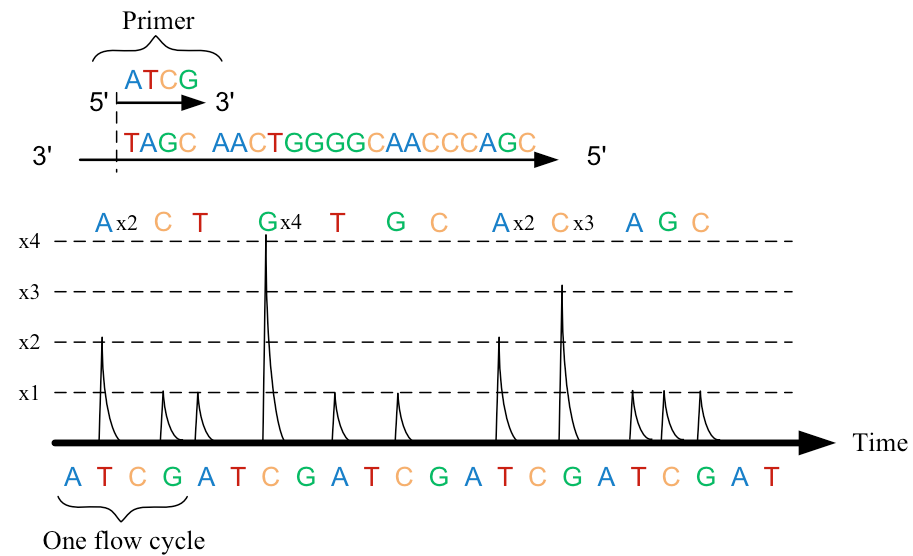
\includegraphics[width=0.75\textwidth]{./figs/pyrosequencing.png}
  \caption{Pyrosequencing, Diagram by Y Hu \cite{hu2012cmos}}
  \label{fig:pyro}
\end{figure}
This reaction releases both pyrophosphate and a positively charged hydrogen ion. In some approaches the pyrophosphate is detected using optical methods and the timing of the reaction could be used to identify which base. In newer technologies such as that introduced by Rothberg in 2011, non-optical techniques have been developed which allow much denser packing of detectors on a single chip \cite{rothberg2011integrated}. These techniques use transistor technologies called ion-sensitive field-effect transistors (ISFETS). These ISFET devices can sense a change in the pH of a surrounding solution, the pH of the solution fluctuates when a recombination of a base with its complementary pair happens. The change in pH is sensed by the ISFET and as the supplied base is known, the base in the sequence can be identified \cite{wong2010pg}.


The advantage of methods such as these is the density of detectors, allowing massively parallel sequencing to take place, Rothberg's application had 1.2 million wells on a single chip, each able to detect a nucleotide in parallel. The disadvantage of this system however, is the detection time. The synthesis process involves the introduction of chemicals to the DNA sequence and then for a reaction to occur and the resultant chemicals to reach the detector. This is relatively slow process, taking up to 4 seconds for a single detection cycle to occur \cite{rothberg2011integrated}. As a result, any practical application of this approach would need to use a massively parallel short read length approach. Due to this fact, a chemical process has been adopted to duplicate the DNA multiple times, cut it into small chunks and then use the overlaps of these chunks to recombine the sub-sequences into the full sequence. All NGS technologies share this limitation of read lengths being orders of magnitude shorter than even the shortest genome \cite{miller2010assembly}. This is not a trivial computational problem and a variety of assembly algorithms have been proposed as a solution to this. 


\subsection{Assembly Algorithms}

The problem of recombining sub-sequences into a single full sequence is computationally expensive as all overlaps of a sequence must be identified. A number of methods have been used for this, however there are three main groups. 


The Overlap-Layout-Concensus (OLC) algorithm does an all against all comparison of the sub-sequences and produces a graph of where the sequences overlap, a graph can then be produced organising the sub-sequences into order by how they overlap, at this point it is relatively computationally simple to produce a best-guess full sequence. With enough data it is possible to confidently produce a full sequence that is known to be correct. This method is computational expensive due to the all-against-all comparison required at the beginning of the process. Once the comparison is done, the recombination is a relatively trivial problem to solve. 



The Greedy Graph algorithm shares the first step with the OLC method, using an all-against-all comparison to build a graph to be solved. The disadvantage of the Greedy algorithm however, is that at each stage it picks a locally optimal solution, this means that the order of detection can determine the likelihood getting a given result \cite{hu2012cmos}. 



A significantly different approach to assembly is the De Bruijn method. Used in the Solexa and SOLiD platforms \cite{miller2010assembly}, it produces a graph of sequences where each sequence is a node on the graph and any overlaps above a threshold are directed links on the graph. The advantage of this system is that it does not require the same all against all comparison, as overlaps are built up iteratively, however due to the fact the algorithm srotes a large amount of data on sub-sequences it uses a large amount of memory relative to the other algorithms. 


The problem of assembly algorithms is therefore a matter of both approach and implementation. It is difficult however, to minimise the problem of memory usage in the De Bruijn graph assembly method. The all-against-all comparison is computationally intensive, and in this report a method will be introduced to alleviate these constraints, and attempt to scale an OLC method to produce a real-time sequencer. The method that will be used in this report was introduced by Y Hu et al. in 2012, exploiting parallelism and the detection method to produce a real-time all-against-all comparison engine \cite{hu2012cmos}.
\section{The Comparison Engine}
The comparison engine designed by Y Hu et al. looks to exploit the slow read times of the current DNA detection technologies as well as mitigating the computational complexity of the algorithm through the use of parallelism \cite{hu2012cmos}. The comparison engine works on the principle of a ring network as shown in figure \ref{fig:CE}. The system is comprised of a large number of comparator elements known as pixels. These pixels correspond to the detection pixels from the dense parallel detection technology discussed above. They are specifically designed to work on incomplete data sets in order to maximise the processing that can be completed whilst the DNA detection is still taking place. 
  
Each comparator element gets a single sequence of data fed into it from a data source, it caches this data locally. Once enough data has been cached it starts forwarding the end of this sequence to the next pixel. Each pixel then has its locally cached data and an input sequence from the previous pixel. A comparison is done between these two peices of data and the result is stored in a local overlap library. This overlap library stores all the important data to identify an overlap including the length of the overlap and the sequences which overlap. The accumulation of all the pixels' local libraries form a full overlap database which can be used to form a graph in the Overlap-Layout-Concensus algorithm.


As an extension to this basic algorithm Y Hu designed the individual pixels such that the forwarding ring can forward a compile time modifiable number of strings. For example, when setting the \verb|FIX_LENGTH| parameter to 4, each pixel forwards four sequences to the next pixel in parallel and therefore does 4 comparisons per cycle locally. The advantage of this technique is that a balance can be struck between the number of cycle required to do all the comparisons and the complexity of the local pixel. The structure of this algorithm can be seen in figure \ref{fig:CE}. 

This algorithm was provided in the form of a VHDL project, written to 1993 specification VHDL in a set of several parameterisable modules. It is important to note in this design the data source provided is un-synthesizable, this means that while it is written in VHDL similarly to the rest of the code, however it cannot be implemented on hardware. This is appropriate for simulation but not for any practical application. A key part of any practical implementation would be to replace this block with an interface to allow communication with a data source.

This designs exploits the advantages of parallelism as well as the streaming data source in this application, but a full analysis of its computational complexity must be performed to identify the possible applications of this algorithm. A large amount of this work has been quantified by Y Hu et al in a previous paper \cite{hu2012cmos} . In the following section I perform a simple analysis of the properties of this implementation in terms of its resource requirements on hardware as well as the speed and computation it is capable of doing assuming perfect availability of data and a clock speed that can be set.

\begin{figure}[h]
  \centering
  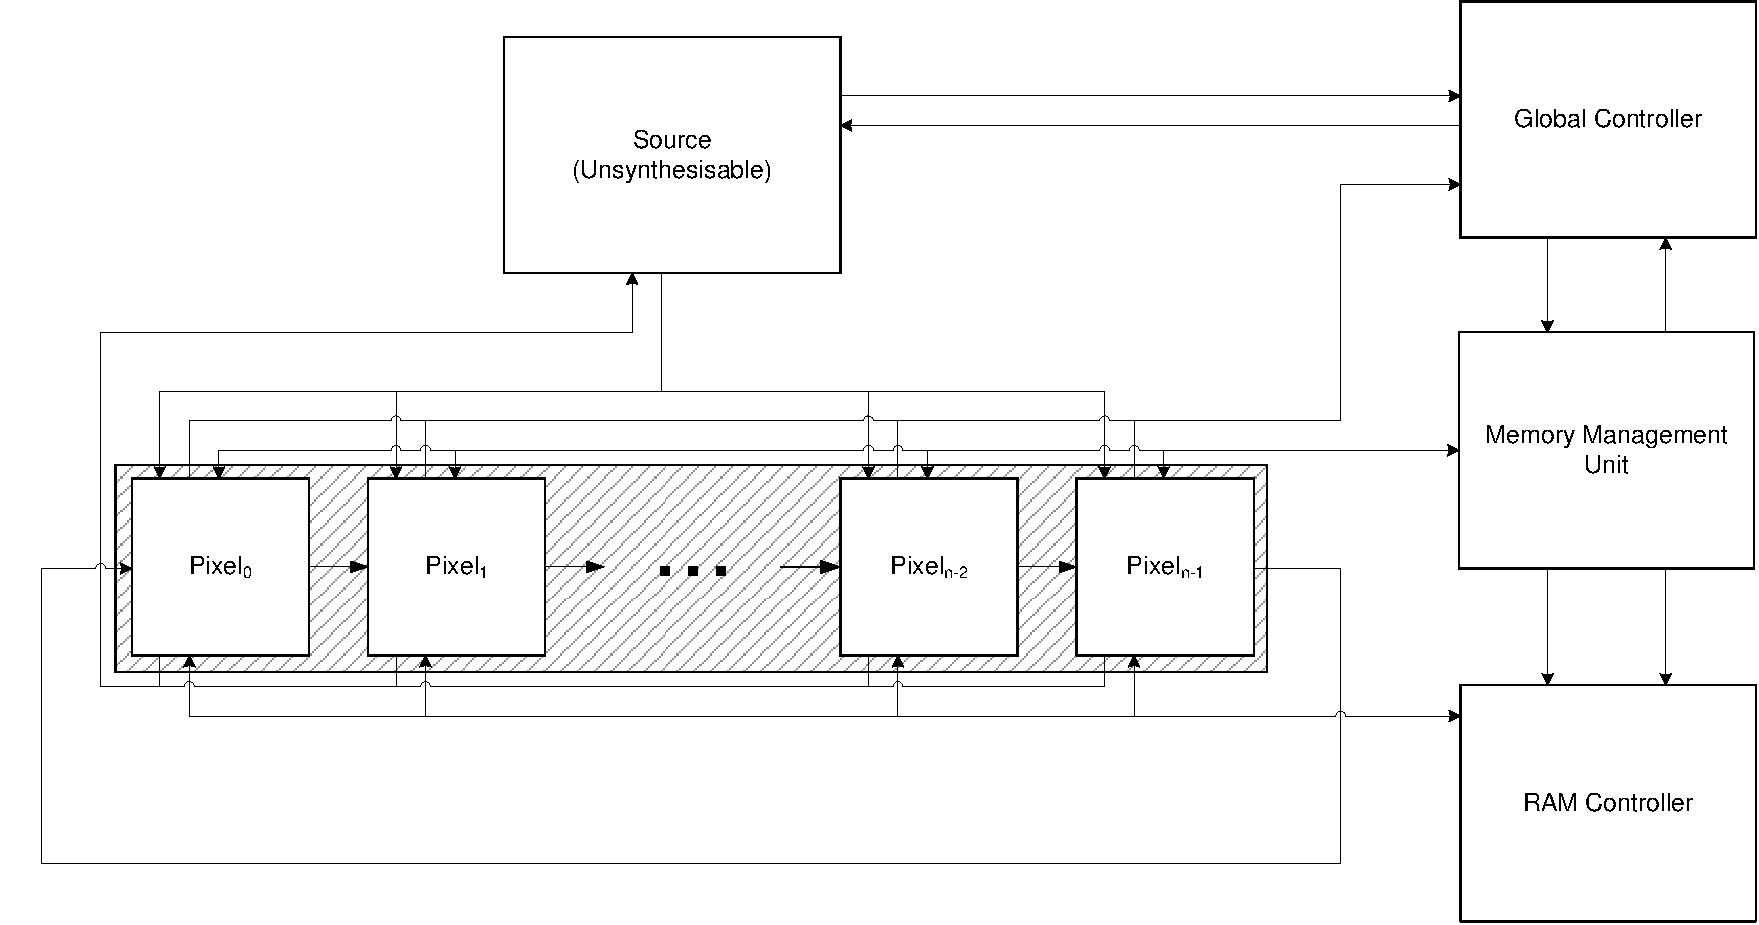
\includegraphics[width=\textwidth]{./figs/UnModified.pdf}
  \caption{Y Hu's Comparison Engine}
  \label{fig:CE}
\end{figure}

\subsection{Complexity Analysis}
The comparison engine algorithm was made available as a VHDL project that fully works in simulation with an included test bench that verifies its functionality. The VHDL implementation provided is a parameterisable project, allowing it to scale with various requirements such as read length, number of pixels and result library size. To give an idea of the scale of the code provided, a set of compilations has been run at different settings. Design size will be listed with 3 factors; Clock frequency shows the speed of design achievable, memory utilisation and logic utilisation show the size of the design.



\begin{table}[!h]
\centering % used for centering table
\begin{tabulary}{\textwidth}{C C C C| C C C}% centered columns (4 columns)
\hline\hline %inserts double horizontal lines
Read Length & Genome Length & Pixel Count & Library Size & Logic Utilisation & Memory Utilisation (Bits) & Frequency (MHz)\\      % inserts table 
%heading
\hline % inserts single horizontal line
50 & 100 & 9 & 3 & 9,916 & 4,096 & 38.5\\ % inserting body of the table
50 & 100 & 9 & 5 & 10,597 & 4,096 & 39.7\\ % inserting body of the table
50 & 100 & 9 & 7 & 11,295 & 4,096 & 39.6 \\ % inserting body of the table
50 & 100 & 9 & 10 & 12,324 & 4,096 & 40.6\\ % inserting body of the table
\hline
50 & 200 & 5 & 5 & 5,896 & 4,096 & 40.2 \\ % inserting body of the table
50 & 200 & 10 & 5 & 11,744 & 4,096 & 40.1\\ % inserting body of the table
50 & 200 & 20 & 5 & 23,590 & 4,096 & 39.5 \\ % inserting body of the table
50 & 200 & 40 & 5 & 50,513 & 4,096 & 34.1\\ % inserting body of the table
\hline
50 & 100 & 5 & 5 & 5,896 & 4,096 & 40.2\\ % inserting body of the table
50 & 1,000 & 5 & 5 & 5,896 & 4,096 & 40.2\\ % inserting body of the table
50 & 10,000 & 5 & 5 & 5,896 & 4,096 & 40.2\\ % inserting body of the table
\hline
100 & 2,000 & 5 & 5 & 5,957  & 4,096 & 41.7\\ % inserting body of the table
200 & 2,000 & 5 & 5 & 6,005 & 4,096 & 41.6\\ % inserting body of the table
400 & 2,000 & 5 & 5 & 6,047 & 4,096 & 41.6\\ % inserting body of the table
800 & 2,000 & 5 & 5 & 6,067 & 4,096 & 41.7\\ % inserting body of the table
1,600 & 2,000 & 5 & 5 & 6,110 & 4,096 & 41.7 \\ % inserting body of the table

\hline
\end{tabulary}
\caption{Design Size of Y Hu's Comparison Engine} % title of Table
\label{table:alg}
\end{table}

These measurements were made on an Altera CYCLONE III device, which is representative of the devices that this algorithm may be built on. As can be seen, logic size primarily scales with pixel count. The overlap library size also has a large effect which is associated with the ratio of read length to genome length as the more reads within the genome will cause more overlaps. Other variables have a much more limited change; the memory utilisation stays constant, as does the frequency. This is because the longest path in the design is held within a single pixel. 


In terms of absolute resources the control logic has very little overhead and the memory utilisation is very low. For any given FPGA, memory generally outnumbers logic elements significantly. In this design, the memory utilisation is very low however, and a fixed level so in this design the logic utilisation will be the limiting factor when fitting the algorithm on to a device.

\section{Hardware Acceleration}

The scope of this project was to build an FPGA accelerator for the comparison process, the reason for the choice of FPGA as the hardware for this project is several fold. The first and most important motivating factor is the reconfigurability of FPGAs, these devices are designed to be reprogrammed many times, allowing the DNA detection hardware to drive the configuration of the comparison engine. This is important due to the many possible ways the DNA detection could be done and the paralellisation of the task. The hardware for this project must also be highly parallelisable in order to take advantage of the pixel based design, a traditional central processing unit (CPU) is by nature serial and therefore could not accelerate the process in the same way. 

General purpose Graphics Processing Units (GPUs) were an alternative to FPGAs in terms of parallelisation, however these are generally not used as stand alone devices and communication between processing units in a GPU can be relatively expensive in terms of performance due the design of the GPU and the hierarchical nature of it's scheduling. Fitting the algorithm to different streaming multi-processors in a GPU would be a necessary complication of that approach. GPUs also have very limited scope for acceleration using additional hardware without complex cluster designs, communicating via protocols such as PCI-Express and this does not favour a ring network design that was discussed earlier. It is expected that FPGA development is a longer process, however the FPGA hardware is tailored perfectly to support the ring network design, allowing massive parallelisation and communication. The FPGA device is also normally a standalone device allowing it to communicate directly with the DNA  detection hardware rather than incurring the cost and delay of a host computer.


The primary motivation for using an FPGA is therefore speed, it has been shown in several papers that FPGAs are capable of signficantly speeding up parallel processess\cite{Fowers:2012:PEC:2145694.2145704}. For suitably parallel applications with large enough problem sizes FPGAs have been shown to be the best solution in terms of performance. This can be seen in figure \ref{fig:cpugpufpga} where for Sum of Absolute Differences (SAD), convolution and Correntropy the FPGA significantly outperforms CPUs and GPUs for most problems\cite{Fowers:2012:PEC:2145694.2145704}. Shown below green represents FPGA, light blue represents GPU accelerated, red represents basic GPU, and dark blue represents CPU.

\begin{figure}[h]
  \centering
  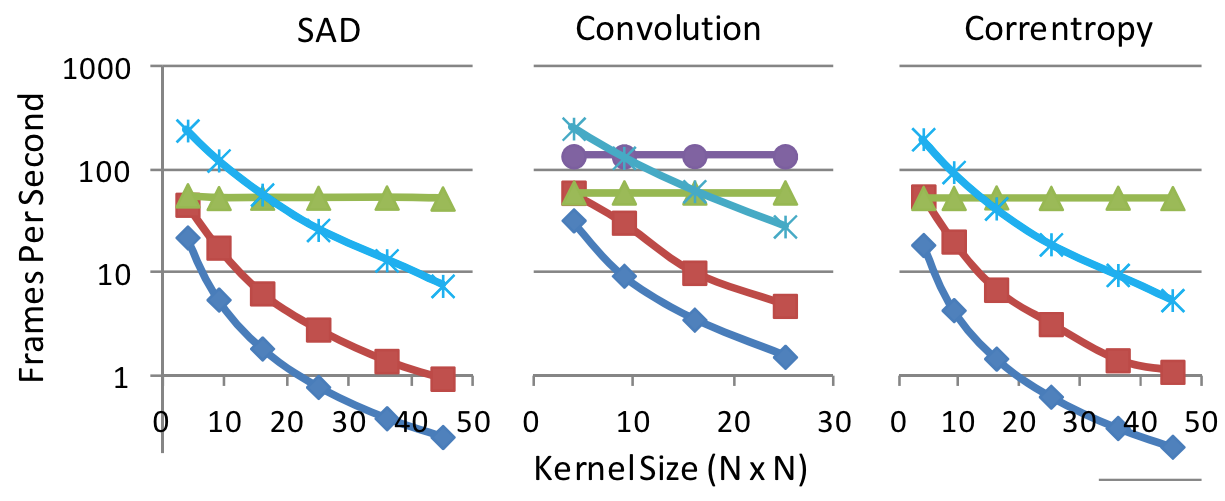
\includegraphics[width=0.7\textwidth]{./figs/cpugpufpga.png}
  \caption{Performance of all implementations in frames per 
second for SAD, 2D Convolution, and correntropy at all kernel 
sizes tested on 720p images. \cite{Fowers:2012:PEC:2145694.2145704}}
  \label{fig:cpugpufpga}
\end{figure}


The only alternative that shares all the benefits of an FPGA  based implementation would be developing an application specific integrated circuit (ASIC). An ASIC would not be easily reconfigurable but would be truly parallel in the ring network's design and could be built on the same chip as the detection hardware. The draw back of this approach however, is the enormous cost and time associated with developing an ASIC).  The design of an FPGA based system also leaves the possibility of an ASIC based implementation at a later point based on the FPGA design.
\vspace*{\fill}


